% Created 2022-06-30 Thu 10:24
% Intended LaTeX compiler: pdflatex
\documentclass[presentation,aspectratio=169]{beamer}
\usepackage[utf8]{inputenc}
\usepackage[T1]{fontenc}
\usepackage{graphicx}
\usepackage{grffile}
\usepackage{longtable}
\usepackage{wrapfig}
\usepackage{rotating}
\usepackage[normalem]{ulem}
\usepackage{amsmath}
\usepackage{textcomp}
\usepackage{amssymb}
\usepackage{capt-of}
\usepackage{hyperref}
\usepackage{khpreamble}
\usepackage{amssymb}
\DeclareMathOperator{\shift}{q}
\DeclareMathOperator{\diff}{p}
\usepackage{tcolorbox}
\usetheme{default}
\author{Kjartan Halvorsen}
\date{2022-06-30}
\title{From analog to discrete-time systems}
\hypersetup{
 pdfauthor={Kjartan Halvorsen},
 pdftitle={From analog to discrete-time systems},
 pdfkeywords={},
 pdfsubject={},
 pdfcreator={Emacs 26.3 (Org mode 9.4.6)}, 
 pdflang={English}}
\begin{document}

\maketitle

\section{Intro}
\label{sec:org72215e0}


\section{Discrete-time system example}
\label{sec:org2998baa}

\section{Zero-order hold, or step-invariant sampling preview}
\label{sec:orge96f1c7}

\begin{frame}[label={sec:org7315fe8}]{The world according to the discrete-time controller}
\begin{center}
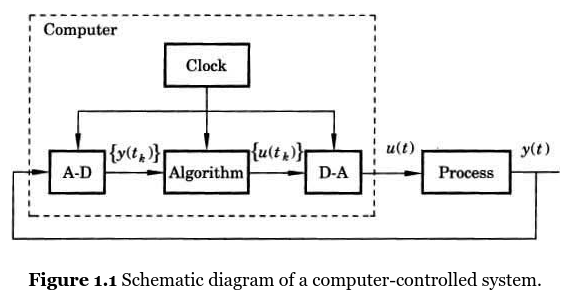
\includegraphics[width=0.6\linewidth]{../../figures/fig1-1-schematic.png} Source: Åström and Wittenmark "Computer-controlled systems".
\end{center}
\end{frame}

\begin{frame}[label={sec:org0ba1e00}]{Discrete-time Linear Shift-Invariant systems}
\small

\begin{center}
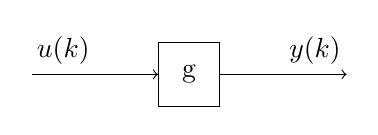
\begin{tikzpicture}[scale=0.6,node distance=20mm, anchor=north]
\node[coordinate] (input) {};
\node[rectangle, draw, right of=input, inner sep=3mm] (lti) {g};
\node[coordinate, right of=lti] (output) {};
\draw[->] (input) -- node[near start, above] {$u(k)$}  (lti);
\draw[->] (lti) -- node[near end, above] {$y(k)$} (output);
\end{tikzpicture}
\end{center}

\pause

\alert{General case (non-causal)}

\begin{align*}
 y(k) &= g \ast u = \sum_{n=-\infty}^\infty g(n) u(k-n)\\ &= \cdots + g(-2)u(k+2) + g(-1)u(k+1) + g(0)u(k) + g(1)u(k-1) + \cdots
 \end{align*}

\pause

\alert{Causal case}
\begin{align*}
 y(k) &= g \ast u = \sum_{n=0}^\infty g(n) u(k-n) \\
 &= g(0)u(k) + g(1)u(k-1) + g(2)u(k-2) + g(3)u(k-3) + \cdots
 \end{align*}


\(g(k)\) is called the \alert{weighting sequence}.
\end{frame}


\begin{frame}[label={sec:org143523b}]{Discrete-time LSI systems}
\begin{block}{Impulse response}
If the input signal is a unit discrete impulse

\begin{center}
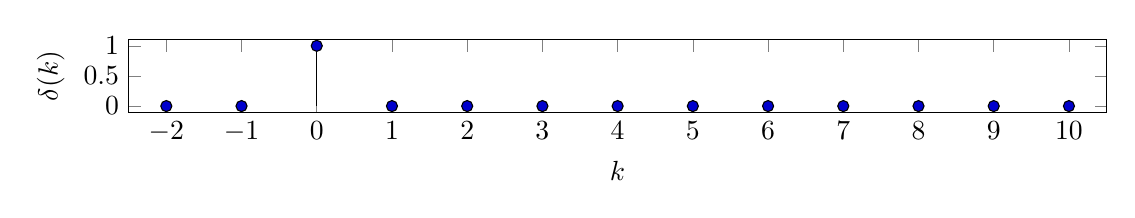
\begin{tikzpicture}
\begin{axis}[
  width=14cm,
  height=2.5cm,
  xlabel={$k$},
  ylabel={$\delta(k)$},
  xmin=-2.5,
  xmax=10.5,
]

\addplot+[black, ycomb, domain=-2:10, samples=13,variable=k] { (k==0)}; 

\end{axis}
\end{tikzpicture}
\end{center}

\pause

\[ y(k) = \sum_{n=0}^\infty g(n) \delta(k-n) = g(k) \]

\alert{The weighting sequence is equal to the impulse response of the system.}
\end{block}
\end{frame}

\begin{frame}[label={sec:org577acfc}]{The response of a discrete LSI system is a weighted sum of the current and previous values of the input}
\small 

\[ y(k) = g \ast u = \sum_{n=0}^\infty g(n) u(k-n) = g(0)u(k) + g(1)u(k-1) + g(2)u(k-2) + \cdots \]


\alert{Activity} What is the response of a system to the input signal \(u(k)\) if its impulse response (weighting sequence) is the one below?

\begin{center}
\begin{tikzpicture}
\small
\begin{axis}[
  width=14cm,
  height=3.5cm,
  xlabel={$k$},
  ylabel={$g(k)$},
  xmin=-0.5,
  xmax=10.5,
  ytick = {0, 1},
]

\addplot+[black, ycomb, domain=-2:10, samples=13,variable=k] { (k==4)}; 

\end{axis}
\end{tikzpicture}
\end{center}

\[y(k) = \]
\end{frame}


\section{The z-transform}
\label{sec:org2fdb3a4}
\begin{frame}[label={sec:org4e5859c}]{The Laplace transform}
\begin{block}{Definition}
\[ F(s) = \laplace{f(t)} = \int_0^\infty f(t) \mathrm{e}^{-st} dt\]
\end{block}
\begin{block}{Inverse transform}
\[ f(t) = \mathcal{L}^{-1}\{F(s)\} = \frac{1}{2\pi i} \int_{\gamma - i\infty}^{\gamma + i\infty} F(s)\mathrm{e}^{st} \, ds \]

Note that in control engineering, the one-sided transform is used.
\end{block}
\end{frame}

\begin{frame}[label={sec:org465eb16}]{The z-transform}
\begin{block}{Definition}
\[ F(z) = \ztrf{f(kh)} = \sum_{k=0}^{\infty} f(kh)z^{-k} \]
\end{block}

\begin{block}{Inverse transform}
\[ f(kh) = \frac{1}{2\pi i} \oint_r F(z) z^{k-1} \, dz \]

Note that in control engineering, the one-sided transform is used.
\end{block}
\end{frame}

\begin{frame}[label={sec:org52e8fce}]{The Laplace transform of a sampled signal}
Assume right-sided signal \(f(t)\), meaning it is zero for negative times \(t<0\).
\[f_s(t) = f(t)m(t) = f(t) \sum_{k=0}^{\infty} \delta(t-kh) = \sum_{k=0}^{\infty} f(t)\delta(t-kh) = \sum_{k=0}^{\infty} f(kh) \delta(t-kh) \]

\pause

\begin{align*}
F_s(s) &= \laplace{f_s(t)} = \int_0^\infty \left(\sum_{k=0}^{\infty} f(kh) \delta(t-kh)\right)\mathrm{e}^{-st}\, dt \\
&= \sum_{k=0}^{\infty} \int_0^\infty  f(kh) \delta(t-kh) \mathrm{e}^{-st}\, dt = \sum_{k=0}^{\infty} f(kh) \mathrm{e}^{-skh}\\
&= \sum_{k=0}^{\infty} f(kh) \left(\mathrm{e}^{sh}\right)^{-k}
\end{align*}
\end{frame}

\begin{frame}[label={sec:orgc661961}]{The Laplace transform of a sampled signal}
Note:
\begin{align*}
F_s(s) &=  \sum_{k=0}^{\infty} f(kh) \left(\mathrm{e}^{sh}\right)^{-k}\quad \text{Laplace transform}\\
F(z) &= \sum_{k=0}^{\infty} f(kh) z^{-k} \quad \text{z-transform}
\end{align*}

\begin{tcolorbox}
 The z-transform of a sampled signal corresponds to its Laplace transform with the following relationship between the s-plane of the Laplace transform and the z-plane of the z-plane of the z-transform.
\[ z = \mathrm{e}^{sh}\]
\end{tcolorbox}
\end{frame}

\begin{frame}[label={sec:org2067d75}]{Exercise on the z-transform}
\small

\begin{center}
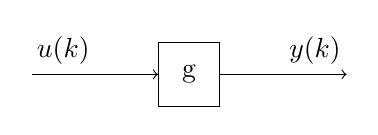
\begin{tikzpicture}[scale=0.6,node distance=20mm, anchor=north]
\node[coordinate] (input) {};
\node[rectangle, draw, right of=input, inner sep=3mm] (lti) {g};
\node[coordinate, right of=lti] (output) {};
\draw[->] (input) -- node[near start, above] {$u(k)$}  (lti);
\draw[->] (lti) -- node[near end, above] {$y(k)$} (output);
\end{tikzpicture}
\end{center}

\pause

\[ G(z) &= \sum_{k=0}^{\infty} g(k) z^{-k} \quad \text{z-transform}\]

\alert{Activity} What is the z-transform of the delayed impulse signal \(g(k) = \delta(k-4)\) below?

\begin{center}
\begin{tikzpicture}
\small
\begin{axis}[
  width=14cm,
  height=3.5cm,
  xlabel={$k$},
  ylabel={$g(k)$},
  xmin=-0.5,
  xmax=10.5,
  ytick = {0, 1},
]

\addplot+[black, ycomb, domain=-2:10, samples=13,variable=k] { (k==4)}; 

\end{axis}
\end{tikzpicture}
\end{center}
\end{frame}




\begin{frame}[label={sec:orgc11b3fc}]{One of the most important transform pairs}
\[f(kh) = \alpha^{kh}, \quad \alpha \in \mathbb{C}\]

\pause

\begin{align*}
   F(z) &= \ztrf{f(kh)} = \sum_{k=0}^{\infty} f(kh)z^{-k}
   =  \sum_{k=0}^{\infty} \alpha^{kh}z^{-k} =  \sum_{k=0}^{\infty} \left(\alpha^{h}\right)^kz^{-k}\\
   &=  \sum_{k=0}^{\infty} \left(\frac{\alpha^{h}}{z}\right)^{k}
   =  \frac{1}{1 - \frac{\alpha^h}{z}} = \frac{z}{z-\alpha^{h}}, \quad |\frac{\alpha^h}{z}| < 1
\end{align*}

\pause

\begin{tcolorbox}
\[ \alpha^{kh} \quad  \overset{\mathcal{Z}}{\longleftrightarrow} \quad \frac{z}{z-\alpha^h} \]
\end{tcolorbox}
\end{frame}


\begin{frame}[label={sec:orgcc284a9}]{Step-invariant sampling (a.k.a ZOH sampling)}
\begin{center}
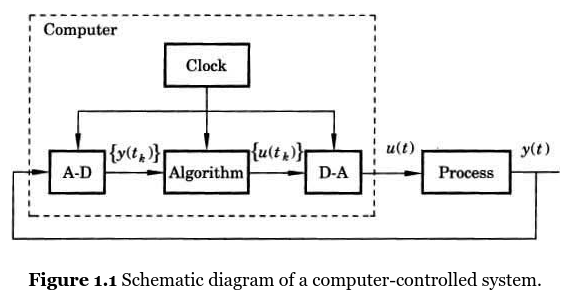
\includegraphics[width=0.6\linewidth]{../../figures/fig1-1-schematic.png} Source: Åström and Wittenmark "Computer-controlled systems".
\end{center}
\end{frame}

\begin{frame}[label={sec:org96db9df}]{Step-invariant sampling (a.k.a ZOH sampling)}
\begin{center}
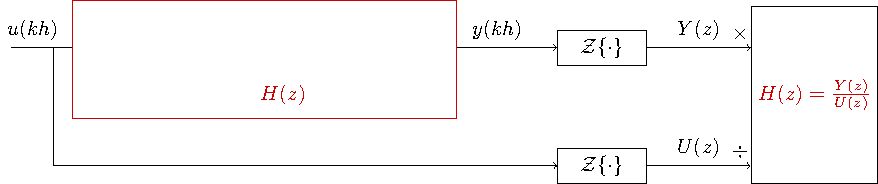
\includegraphics[width=0.9\linewidth]{../../figures/invariant-sampling-white.pdf}
\end{center}

\pause
Step-invariant sampling (zero order hold): \(u(kh) = \begin{cases} 1, & k \ge 0\\0, & k<0 \end{cases}\)
\end{frame}

\begin{frame}[label={sec:org118eb6f}]{Step-invariant sampling (a.k.a ZOH sampling)}
The idea is to sample the continuous-time system's response to a step input, in order to obtain a discrete approximation which is \alert{exact} (at the sampling instants) for such an input signal. 

\begin{center}
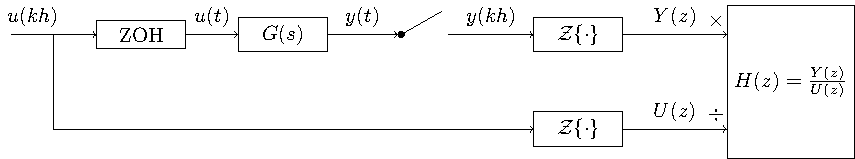
\includegraphics[width=0.9\linewidth]{../../figures/invariant-sampling.pdf}
\end{center}

Step-invariant sampling (zero order hold): \(u(kh) = \begin{cases} 1, & k \ge 0\\0, & k<0 \end{cases}\)
\end{frame}

\begin{frame}[label={sec:org73d5760}]{Why is step-invariant sampling a good idea?}
A piecewise constant (stair-case shaped) function can be written as a sum of delayed step-responses!
\begin{center}
  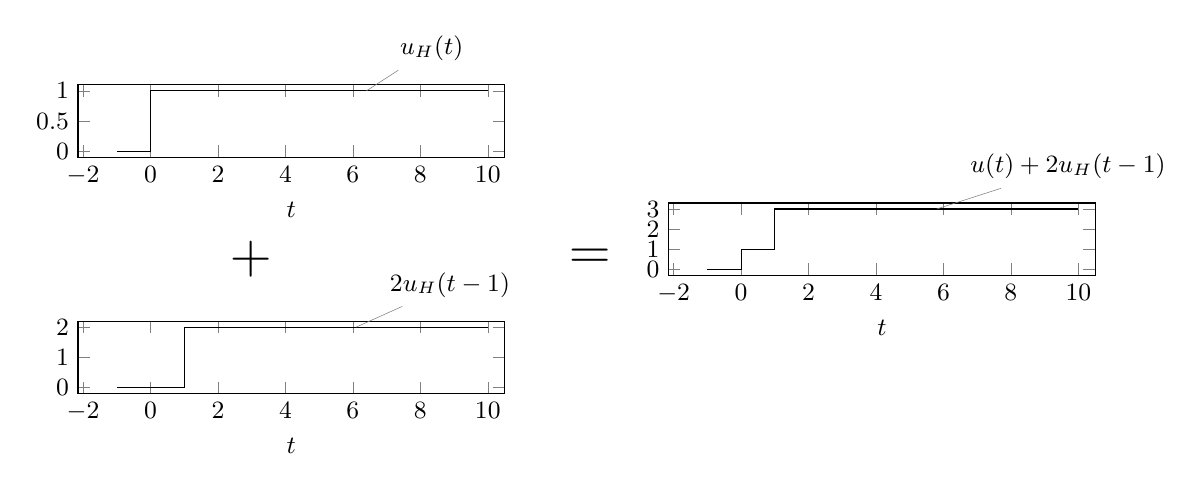
\begin{tikzpicture}
    \small
    \begin{axis}[
      clip = false,
      width=7cm,
      height=2.5cm,
      yshift=1.5cm,
      xlabel={$t$},
      ylabel={},
      xmax=10.5,
      ]
      \addplot+[black, no marks] coordinates {(-1,0) (0,0) (0,1) (10,1) } node[pos=0.7,coordinate, pin=40:$u_H(t)$] {};
    \end{axis}
    \begin{axis}[
      clip=false,
      width=7cm,
      height=2.5cm,
      yshift=-1.5cm,
      xlabel={$t$},
      ylabel={},
      xmax=10.5,
      ]
      \addplot+[black, no marks] coordinates {(-1,0) (1,0) (1,2) (10,2) } node[pos=0.7,coordinate, pin=40:$2u_H(t-1)$] {};;
    \end{axis}
    \begin{axis}[
      clip=false,
      width=7cm,
      height=2.5cm,
      xshift=7.5cm,
      xlabel={$t$},
      ylabel={},
      xmax=10.5,
      ]
      \addplot+[black, no marks] coordinates {(-1,0) (0,0) (0,1) (1,1) (1,3) (10,3) }  node[pos=0.7,coordinate, pin=40:$u(t) + 2u_H(t-1)$] {};;
    \end{axis}

    \node at (2.2,0.2) {\huge  +};
    \node at (6.5,0.2) {\huge  =};

  \end{tikzpicture}
\end{center}
\end{frame}

\section{The z-transform}
\label{sec:org34fba72}

\section{Zero-order hold sampling procedure}
\label{sec:org452b0e5}
\begin{frame}[label={sec:orgd344fa3}]{Step-invariant sampling, or zero-order-hold sampling}
Let the input to the continuous-time system be a unit step \(u(t)=u_H(t),\) which has Laplace transform \(U(s)=\frac{1}{s}.\) In the Laplace-domain we get
\[Y(s) = G(s)\frac{1}{s}\]
\begin{enumerate}
\item Obtain the time-response by inverse Laplace: \(y(t)=\laplaceinv{Y(s)}\)
\item Sample the time-response to obtain the sequence \(y(kh)\) and apply  the z-transform to obtain \(Y(z) = \ztrf{y(kh)}\)
\item Calculate the pulse-transfer function by dividing with the z-transform of the input signal \(U(z) = \frac{z}{z-1}.\) \[H(z) = \frac{Y(z)}{U(z)} = \frac{z-1}{z}Y(z) \]
\end{enumerate}
\end{frame}
\end{document}